\documentclass[10pt,a4paper]{article}
\usepackage[margin=1.8cm]{geometry}
\usepackage[T1]{fontenc}\usepackage[utf8]{inputenc}\usepackage{lmodern}
\usepackage{booktabs,graphicx,float,amsmath,xcolor,hyperref,textcomp}
\DeclareUnicodeCharacter{20AC}{\texteuro}\DeclareUnicodeCharacter{2212}{-}
\hypersetup{colorlinks,linkcolor=blue}
\setlength{\parindent}{0pt}\setlength{\parskip}{4pt}
\title{\textbf{OAT hazard-rate relative value}\\\large Result sheet, run \texttt{R25\_k5}}
\author{Octave, Master 203 thesis project (\texttt{oat-hazard-rv})}
\date{Generated 24 November 2026}
\begin{document}\maketitle


\section*{Setup}
Sample 2010-01-08 to 2026-11-24, 882 fit dates (weekly (Friday)),
117 distinct fixed-coupon OATs, 46 bonds per date (median).
Main run: recovery $R=25\%$ of face, hazard buckets starting at 0,3,7,15,30 years,
negative $\lambda$ allowed so that the QE breakdown is visible. Risk-free curve: €STR OIS
(EONIA OIS $-8.5$bp before Oct 2019).
\[
P=\sum_i CF_i\,D(t_i)\,Q(t_i)+100R\sum_k D(m_k)\big[Q(m_{k-1})-Q(m_k)\big],\qquad
Q(t)=e^{-\int_0^t\lambda},\qquad s\approx\lambda(1-R).
\]
Residual $=$ market yield $-$ model yield (bp, $>0$ = cheap). Baseline: Z-spread minus a cubic in maturity.

\textbf{Real Bloomberg data} (pulled 24 Nov 2026): 117 fixed-coupon nominal OATs, 2010 to today, weekly fits. Main specification: recovery 25\% and five hazard buckets (0-3, 3-7, 7-15, 15-30, 30Y+). Recovery 40\% cannot price the deep-discount ultra-long OATs (0.5\% 2072 at 23, 0.75\% 2053 at 37). \textbf{Funding:} French GC repo history is not entitled on the terminal used; STOXX GC Pooling (ECB basket) sits within a few bp of €STR and changes nothing. Using 3M BTF bills minus €STR as a collateral-scarcity proxy (comparison run R25\_k5\_fundbtf) cuts the share of QE dates where the fit wants $\lambda<0$ from 77\% to 40\%, and lifts the average 0-3Y $\lambda$ under QE from $-12$bp to $+3$bp.

\section{Data}
Figure~\ref{fig:data} shows the last cross-section; Table~\ref{tab:snap} lists every bond in it
(also saved as \texttt{data\_snapshot.csv}).
\begin{figure}[H]\centering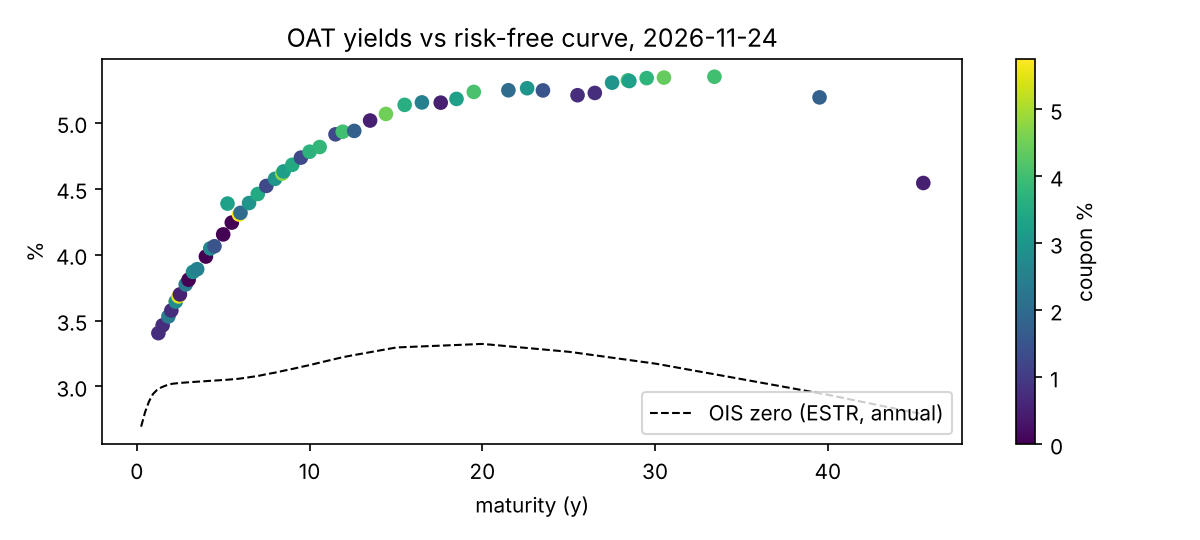
\includegraphics[width=0.85\linewidth]{fig_data.png}\caption{Cross-section on 2026-11-24.}\label{fig:data}\end{figure}
\begin{table}[H]\centering\small
\caption{Market inputs on 2026-11-24}
\begin{tabular}{lrl}\toprule
\textbf{Input} & \textbf{Value} & \textbf{Unit} \\ \midrule
Overnight (€STR) & 2.443 & \% \\
GC repo − €STR & 7.800 & bp \\
OIS zero 2Y (ESTR) & 2.975 & \% \\
OIS zero 5Y (ESTR) & 3.002 & \% \\
OIS zero 10Y (ESTR) & 3.113 & \% \\
OIS zero 30Y (ESTR) & 3.124 & \% \\
GDBR10 generic yield & 3.268 & \% \\
GFRN10 generic yield & 4.783 & \% \\
France CDS 1Y (USD) & 41.728 & bp \\
France CDS 3Y (USD) & 68.086 & bp \\
France CDS 5Y (USD) & 90.629 & bp \\
France CDS 7Y (USD) & 109.774 & bp \\
France CDS 10Y (USD) & 129.638 & bp \\
\bottomrule\end{tabular}\end{table}

\begin{table}[H]\centering\footnotesize
\caption{\label{tab:snap}OAT cross-section on 2026-11-24}
\begin{tabular}{lrrrrrrrr}\toprule
\textbf{ISIN} & \textbf{Cpn \%} & \textbf{Maturity} & \textbf{Clean} & \textbf{YTM \%} & \textbf{ModDur} & \textbf{Z (bp)} & \textbf{Z resid} & \textbf{Haz resid} \\ \midrule
FR001400AIN5 & 0.75 & 2028-02-25 & 96.80 & 3.40 & 1.20 & 41.14 & -9.98 & -18.94 \\
FR0013286192 & 0.75 & 2028-05-25 & 96.11 & 3.46 & 1.44 & 44.60 & -10.34 & -15.32 \\
FR001400XLW2 & 2.40 & 2028-09-24 & 98.03 & 3.53 & 1.74 & 49.72 & -10.29 & -10.39 \\
FR0013341682 & 0.75 & 2028-11-25 & 94.64 & 3.58 & 1.92 & 53.46 & -9.09 & -5.96 \\
FR001400HI98 & 2.75 & 2029-02-25 & 98.09 & 3.64 & 2.09 & 59.75 & -6.51 & -0.05 \\
FR0000571218 & 5.50 & 2029-04-25 & 104.09 & 3.68 & 2.18 & 63.53 & -5.08 & 2.96 \\
FR0013407236 & 0.50 & 2029-05-25 & 92.51 & 3.70 & 2.39 & 64.61 & -5.18 & 5.84 \\
FR0014016G71 & 2.40 & 2029-09-24 & 96.37 & 3.77 & 2.66 & 71.66 & -2.87 & 12.51 \\
FR0013451507 & 0.00 & 2029-11-25 & 89.40 & 3.81 & 2.89 & 74.89 & -2.01 & 16.91 \\
FR001400PM68 & 2.75 & 2030-02-25 & 96.64 & 3.87 & 2.97 & 80.53 & 0.17 & 11.14 \\
FR0011883966 & 2.50 & 2030-05-25 & 95.53 & 3.89 & 3.22 & 82.35 & -1.29 & 4.53 \\
FR0013516549 & 0.00 & 2030-11-25 & 85.54 & 3.99 & 3.84 & 91.14 & 0.89 & -0.14 \\
FR001400Z2L7 & 2.70 & 2031-02-25 & 94.83 & 4.05 & 3.83 & 96.97 & 3.50 & -0.39 \\
FR0012993103 & 1.50 & 2031-05-25 & 89.66 & 4.06 & 4.17 & 98.31 & 1.79 & -3.86 \\
FR0014002WK3 & 0.00 & 2031-11-25 & 81.60 & 4.15 & 4.80 & 106.49 & 3.83 & -3.84 \\
FR0014018OI0 & 3.25 & 2032-02-25 & 95.55 & 4.39 & 4.58 & 128.78 & 23.14 & 15.24 \\
FR0014007L00 & 0.00 & 2032-05-25 & 79.59 & 4.24 & 5.27 & 114.28 & 5.78 & -2.61 \\
FR0000187635 & 5.75 & 2032-10-25 & 107.40 & 4.30 & 4.97 & 120.11 & 6.87 & -2.42 \\
FR001400BKZ3 & 2.00 & 2032-11-25 & 87.98 & 4.32 & 5.45 & 121.04 & 6.86 & -1.65 \\
FR001400H7V7 & 3.00 & 2033-05-25 & 92.27 & 4.39 & 5.63 & 127.32 & 7.78 & -0.17 \\
FR001400L834 & 3.50 & 2033-11-25 & 94.34 & 4.46 & 6.03 & 133.11 & 8.34 & 1.65 \\
FR0013313582 & 1.25 & 2034-05-25 & 79.59 & 4.52 & 6.79 & 137.49 & 7.79 & 1.04 \\
FR001400QMF9 & 3.00 & 2034-11-25 & 89.65 & 4.57 & 6.86 & 141.85 & 7.34 & -0.42 \\
FR0010070060 & 4.75 & 2035-04-25 & 100.90 & 4.61 & 6.64 & 144.92 & 6.62 & -1.94 \\
FR001400X8V5 & 3.20 & 2035-05-25 & 90.12 & 4.63 & 7.06 & 146.01 & 6.98 & -0.77 \\
FR0014012II5 & 3.50 & 2035-11-25 & 91.48 & 4.68 & 7.46 & 149.75 & 6.33 & -0.98 \\
FR0013154044 & 1.25 & 2036-05-25 & 73.83 & 4.74 & 8.44 & 152.85 & 5.28 & 0.41 \\
FR0014018YR0 & 3.70 & 2036-11-25 & 91.57 & 4.78 & 8.07 & 156.71 & 5.15 & -0.51 \\
FR0014017Z10 & 3.80 & 2037-06-25 & 91.71 & 4.82 & 8.27 & 158.62 & 2.70 & -1.87 \\
FR0014009O62 & 1.25 & 2038-05-25 & 68.40 & 4.91 & 10.00 & 164.18 & 1.89 & 3.15 \\
FR0010371401 & 4.00 & 2038-10-25 & 91.75 & 4.93 & 9.11 & 166.44 & 1.43 & 0.18 \\
FR0013234333 & 1.75 & 2039-06-25 & 70.64 & 4.94 & 10.49 & 164.40 & -4.67 & -0.69 \\
FR0013515806 & 0.50 & 2040-05-25 & 56.47 & 5.02 & 12.23 & 168.84 & -5.33 & 5.17 \\
FR0010773192 & 4.50 & 2041-04-25 & 94.27 & 5.07 & 10.00 & 174.83 & -3.89 & 0.30 \\
FR001400WYO4 & 3.60 & 2042-05-25 & 83.84 & 5.14 & 10.97 & 179.54 & -3.89 & 3.06 \\
FR001400CMX2 & 2.50 & 2043-05-25 & 70.97 & 5.15 & 12.23 & 180.00 & -7.15 & 1.87 \\
FR0014002JM6 & 0.50 & 2044-06-25 & 47.04 & 5.15 & 15.55 & 177.16 & -13.42 & 3.41 \\
FR0011461037 & 3.25 & 2045-05-25 & 77.35 & 5.18 & 12.57 & 182.14 & -10.84 & -5.31 \\
FR0014015MU5 & 4.10 & 2046-05-25 & 86.32 & 5.23 & 12.35 & 187.33 & -7.81 & -5.46 \\
FR0013257524 & 2.00 & 2048-05-25 & 58.72 & 5.25 & 15.16 & 187.95 & -10.14 & -0.07 \\
FR001400NEF3 & 3.00 & 2049-06-25 & 70.50 & 5.26 & 14.40 & 190.92 & -8.09 & -3.99 \\
FR0013404969 & 1.50 & 2050-05-25 & 50.07 & 5.25 & 16.94 & 189.25 & -10.20 & 3.10 \\
FR0013480613 & 0.75 & 2052-05-25 & 37.85 & 5.21 & 20.12 & 187.53 & -11.95 & 9.37 \\
FR0014004J31 & 0.75 & 2053-05-25 & 36.56 & 5.23 & 20.65 & 190.67 & -8.39 & 13.57 \\
FR001400FTH3 & 3.00 & 2054-05-25 & 67.03 & 5.30 & 15.80 & 199.29 & 0.89 & -0.29 \\
FR0010171975 & 4.00 & 2055-04-25 & 80.83 & 5.32 & 14.94 & 201.73 & 4.11 & -5.39 \\
FR001400OHF4 & 3.25 & 2055-05-25 & 69.99 & 5.32 & 15.74 & 201.45 & 3.90 & -0.60 \\
FR001400XJJ3 & 3.75 & 2056-05-25 & 76.64 & 5.34 & 15.43 & 204.36 & 7.85 & -1.94 \\
FR0014016CV2 & 4.40 & 2057-05-25 & 85.94 & 5.34 & 15.10 & 205.56 & 10.23 & -7.47 \\
FR0010870956 & 4.00 & 2060-04-25 & 79.17 & 5.35 & 15.87 & 209.53 & 18.19 & -9.99 \\
FR0013154028 & 1.75 & 2066-05-25 & 42.67 & 5.19 & 20.63 & 205.61 & 22.22 & 3.66 \\
FR0014001NN8 & 0.50 & 2072-05-25 & 22.79 & 4.54 & 31.38 & 162.29 & -19.46 & 1.41 \\
\bottomrule\end{tabular}\end{table}

\begin{figure}[H]\centering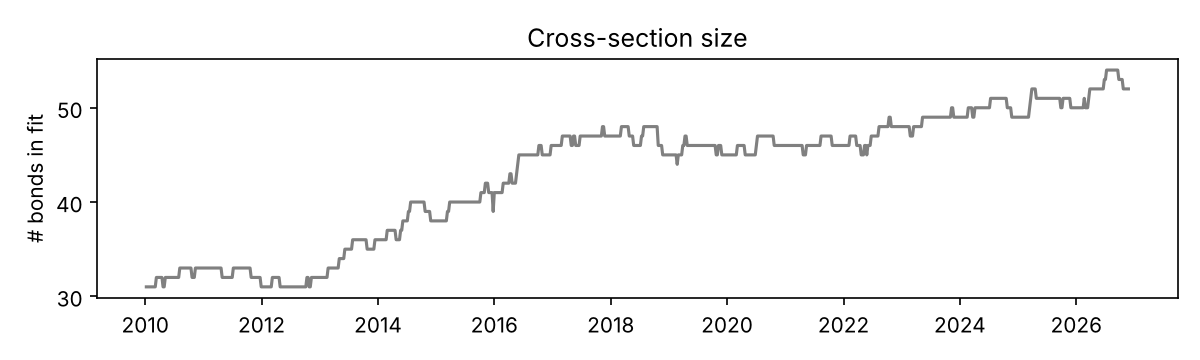
\includegraphics[width=0.85\linewidth]{fig_universe.png}\end{figure}

\section{Fitted credit curve}
\begin{table}[H]\centering\small
\caption{Fitted hazard rates on 2026-11-24}
\begin{tabular}{lrr}\toprule
\textbf{Bucket} & \textbf{Lambda (bp)} & \textbf{Spread approx. (bp)} \\ \midrule
0-3Y & 79.6 & 59.7 \\
3-7Y & 258.8 & 194.1 \\
7-15Y & 317.3 & 238.0 \\
15-30Y & 421.6 & 316.2 \\
30Y+ & 776.8 & 582.6 \\
\bottomrule\end{tabular}\end{table}

\begin{table}[H]\centering\small
\caption{Bond-implied vs traded France CDS (last date). Traded CDS is USD-denominated.}
\begin{tabular}{lrrr}\toprule
\textbf{Tenor} & \textbf{Implied (bp)} & \textbf{Market (bp)} & \textbf{Basis (bp)} \\ \midrule
1Y & 59.1 & 41.7 & -17.4 \\
3Y & 59.1 & 68.1 & 9.0 \\
5Y & 108.8 & 90.6 & -18.1 \\
7Y & 129.6 & 109.8 & -19.9 \\
10Y & 155.4 & 129.6 & -25.8 \\
\bottomrule\end{tabular}\end{table}

\begin{figure}[H]\centering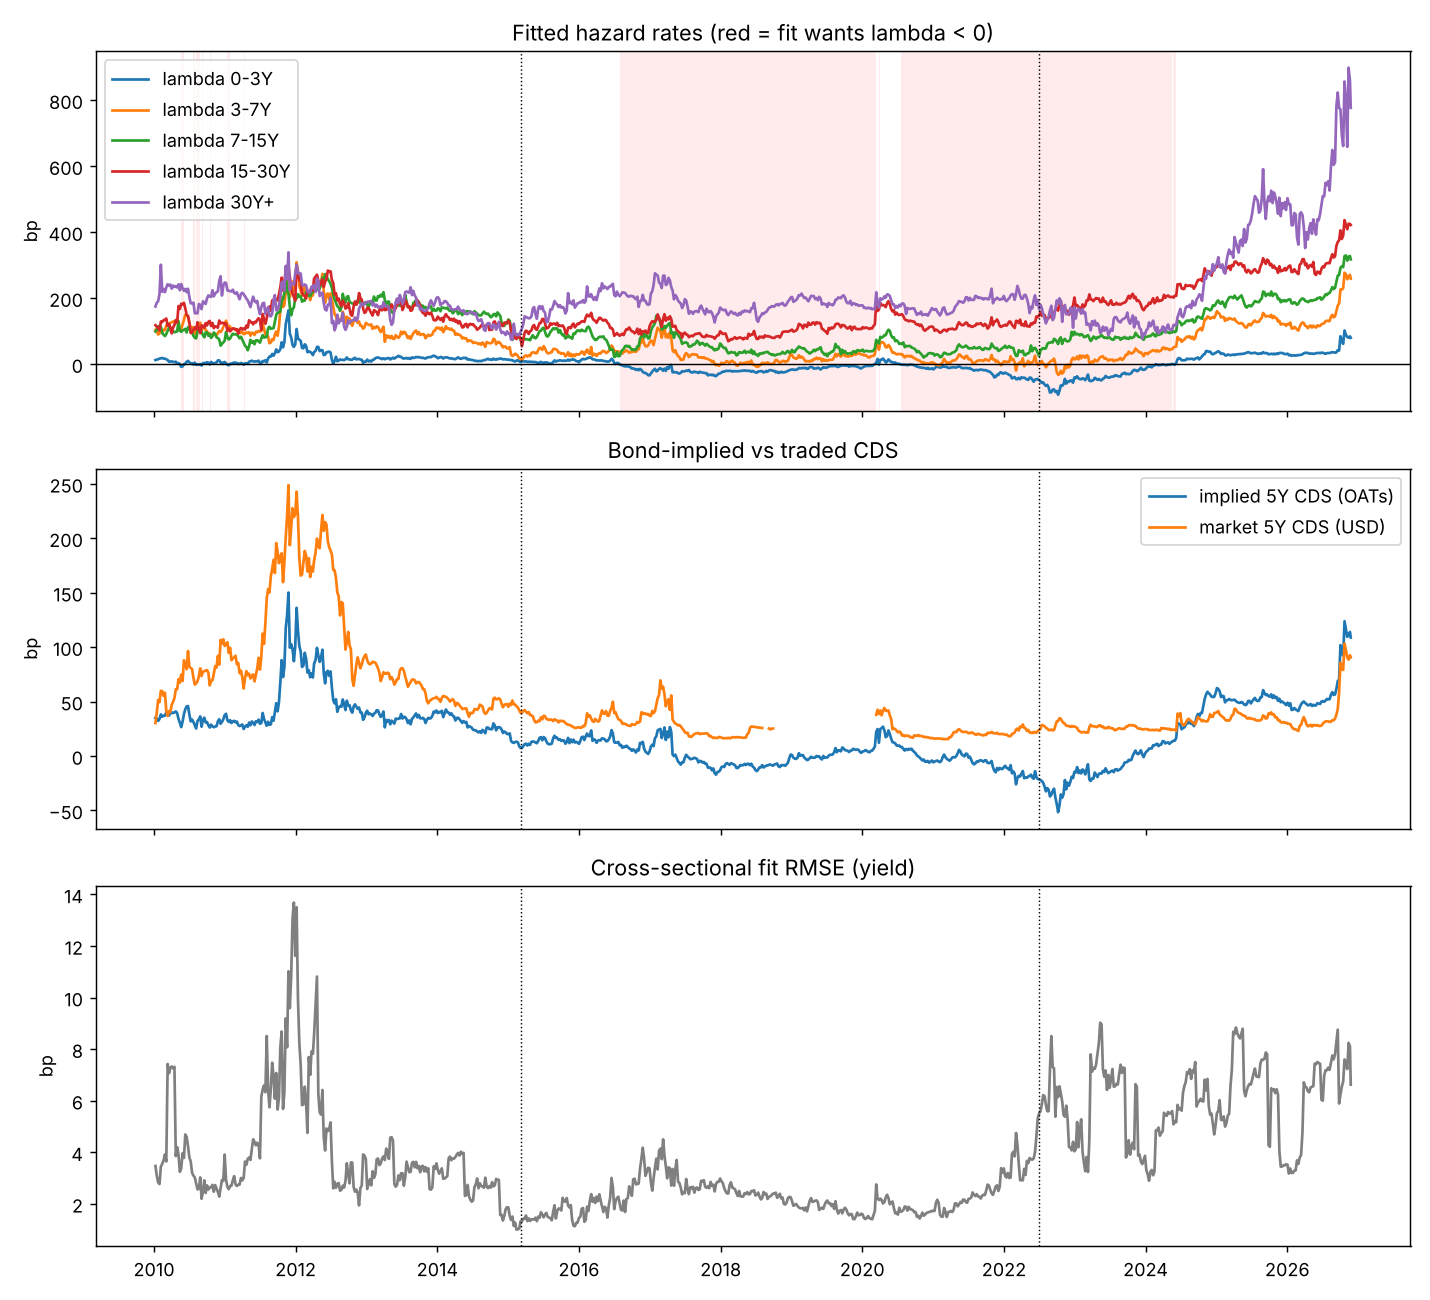
\includegraphics[width=0.95\linewidth]{fig_history.png}
\caption{Run \texttt{R25\_k5}: hazard rates (red = fit wants $\lambda<0$), implied vs traded 5Y CDS, fit RMSE. Dotted lines: QE start (Mar 2015) and end of net purchases (Jun 2022).}\end{figure}
\begin{table}[H]\centering\small
\caption{Fit quality by regime, run R25\_k5}
\begin{tabular}{lrrrrr}\toprule
\textbf{Regime} & \textbf{Dates} & \textbf{Median RMSE (bp)} & \textbf{Share lambda<0} & \textbf{Implied 5Y (bp)} & \textbf{Market 5Y (bp)} \\ \midrule
all & 882 & 3.00 & 0.46 & 19.88 & 50.33 \\
pre-QE & 270 & 3.36 & 0.04 & 41.48 & 91.80 \\
QE & 381 & 2.16 & 0.77 & 1.73 & 27.06 \\
post-QE & 231 & 6.18 & 0.43 & 24.56 & 32.28 \\
\bottomrule\end{tabular}\end{table}


\subsection*{Comparison run \texttt{R25\_k5\_fundbtf}}
\begin{table}[H]\centering\small
\caption{Fit quality by regime, run R25\_k5\_fundbtf}
\begin{tabular}{lrrrrr}\toprule
\textbf{Regime} & \textbf{Dates} & \textbf{Median RMSE (bp)} & \textbf{Share lambda<0} & \textbf{Implied 5Y (bp)} & \textbf{Market 5Y (bp)} \\ \midrule
all & 882 & 3.01 & 0.32 & 24.41 & 50.33 \\
pre-QE & 270 & 3.35 & 0.16 & 43.22 & 91.80 \\
QE & 381 & 2.19 & 0.40 & 12.90 & 27.06 \\
post-QE & 231 & 6.27 & 0.39 & 21.40 & 32.28 \\
\bottomrule\end{tabular}\end{table}

\begin{figure}[H]\centering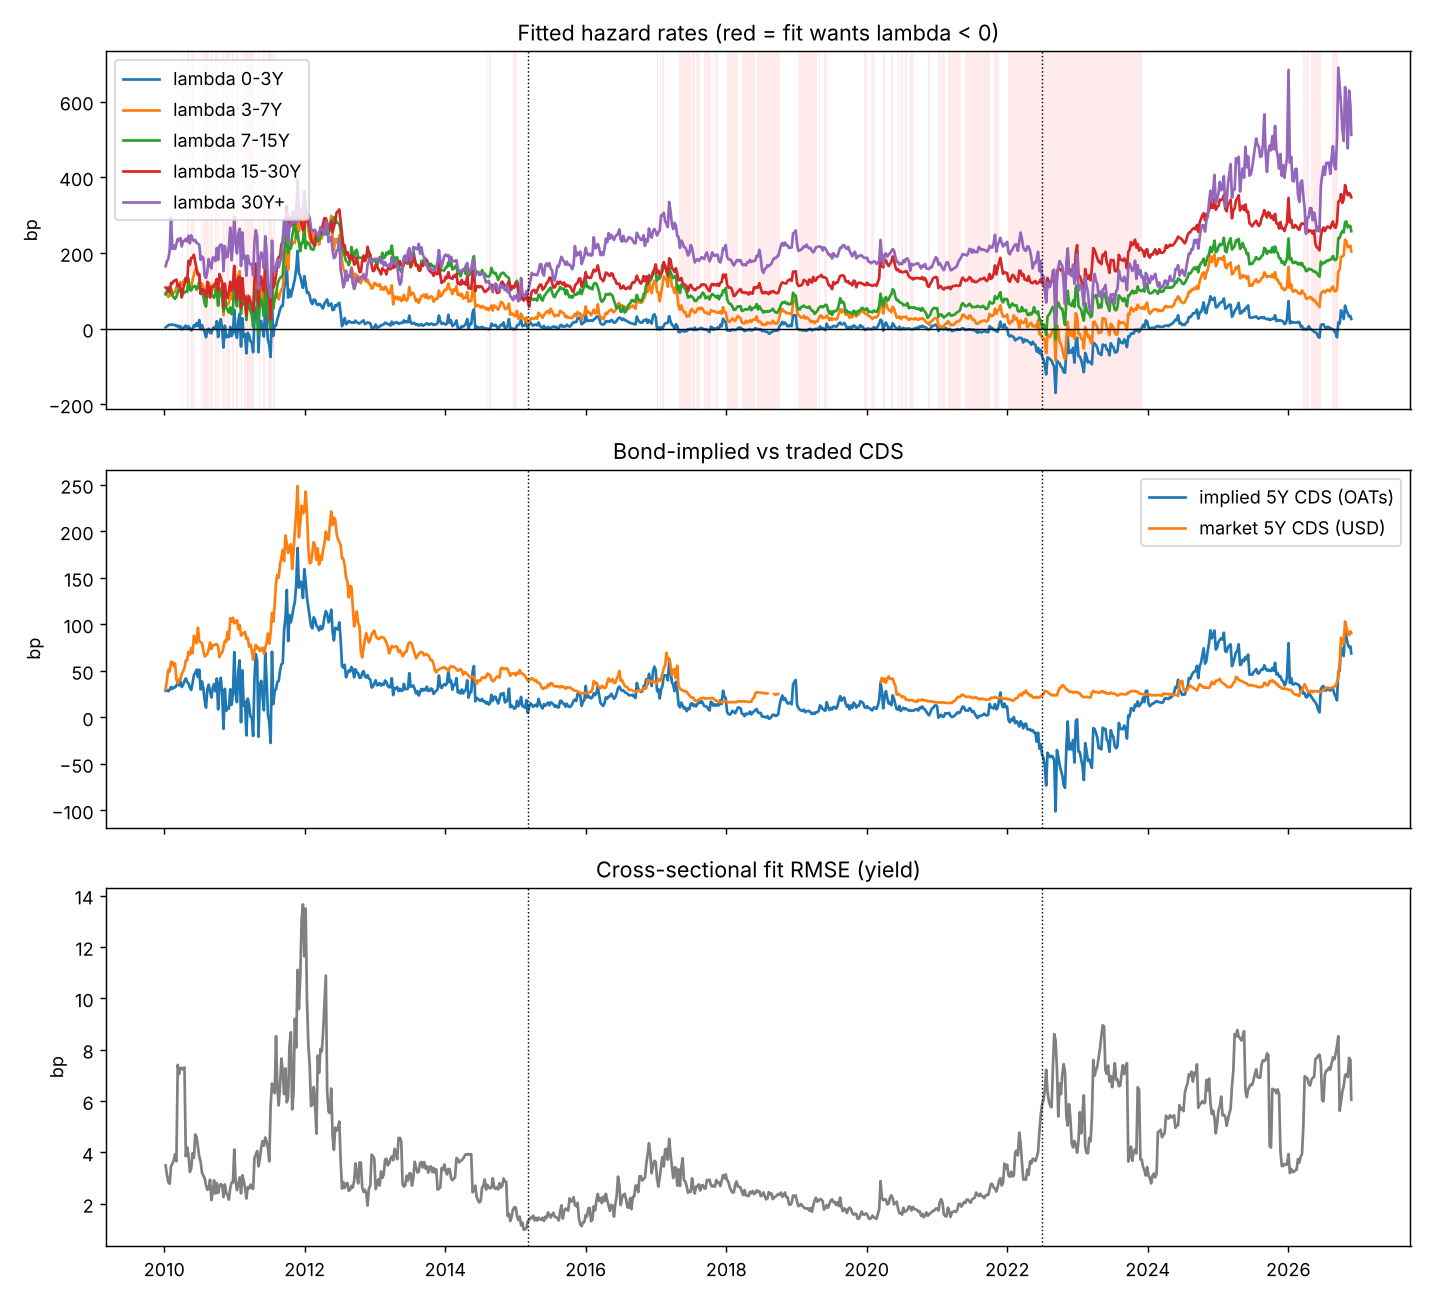
\includegraphics[width=0.95\linewidth]{fig_history_cmp.png}\caption{Run \texttt{R25\_k5\_fundbtf}.}\end{figure}

\section{Sensitivity across specifications}
\begin{table}[H]\centering\footnotesize
\caption{All runs, whole sample. RMSE in bp of yield. Corr(cpn): cross-sectional correlation of the hazard residual with the coupon. IC: rank IC of residual vs next-week compression.}
\resizebox{\linewidth}{!}{\begin{tabular}{llllrrrrrr}\toprule
\textbf{Run} & \textbf{Knots} & \textbf{Recovery} & \textbf{Base} & \textbf{Med. RMSE} & \textbf{RMSE 2024+} & \textbf{Share lambda<0} & \textbf{Corr(cpn) haz} & \textbf{IC haz} & \textbf{IC Z} \\ \midrule
R25\_k5 & 0,3,7,15,30 & 25\% & €STR OIS & 3.000 & 6.300 & 0.457 & -0.071 & 0.112 & 0.095 \\
R25\_k5\_fundbtf & 0,3,7,15,30 & 25\% & €STR OIS & 3.013 & 6.288 & 0.324 & -0.108 & 0.110 & 0.095 \\
R25\_k5\_funding & 0,3,7,15,30 & 25\% & €STR OIS & 2.990 & 6.330 & 0.514 & -0.050 & 0.114 & 0.095 \\
R40 & 0,3,7 & 40\% & €STR OIS & 5.917 & 13.909 & 0.449 & -0.222 & 0.077 & 0.095 \\
R40\_k5 & 0,3,7,15,30 & 40\% & €STR OIS & 3.246 & 8.689 & 0.457 & -0.225 & 0.102 & 0.095 \\
R10\_k5 & 0,3,7,15,30 & 10\% & €STR OIS & 3.013 & 7.173 & 0.457 & 0.043 & 0.108 & 0.095 \\
Rfit\_k5 & 0,3,7,15,30 & fit (mean 23\%) & €STR OIS & 2.899 & 6.230 & 0.457 & -0.038 & 0.113 & 0.095 \\
R25\_k5\_bund & 0,3,7,15,30 & 25\% & Bund & 2.835 & 6.325 & 0.014 & -0.137 & 0.118 & 0.096 \\
\bottomrule\end{tabular}}\end{table}

\begin{figure}[H]\centering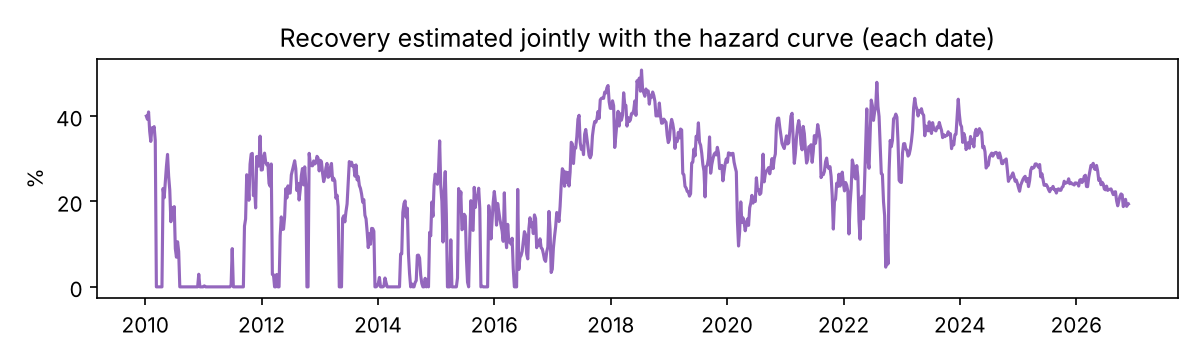
\includegraphics[width=0.85\linewidth]{fig_recovery.png}\end{figure}

\section{Relative-value signals: hazard residual vs Z-spread residual}
Corr(coupon): average cross-sectional correlation with the coupon (Z-spread RV should load on it, the
hazard residual should not). Half-life in fit periods from a pooled AR(1). Rank IC: correlation between the
signal and the next-period residual compression. L/S: long top quintile (cheap), short bottom quintile
(rich), DV01-neutral, residual compression in bp of yield, no carry, roll or costs.
\begin{table}[H]\centering\footnotesize
\caption{Signal comparison, run R25\_k5, horizon 1 period(s)}
\begin{tabular}{lrrrrrrr}\toprule
\textbf{Regime} & \textbf{Signal} & \textbf{Corr(coupon)} & \textbf{Half-life} & \textbf{Rank IC} & \textbf{L/S (bp)} & \textbf{L/S SR} & \textbf{Mean |resid|} \\ \midrule
all & Hazard residual & -0.071 & 15.126 & 0.112 & 0.374 & 0.280 & 2.650 \\
all & Z-spread residual & -0.133 & 14.878 & 0.095 & 0.427 & 0.261 & 3.225 \\
pre-QE & Hazard residual & -0.228 & 12.814 & 0.128 & 0.493 & 0.274 & 2.708 \\
pre-QE & Z-spread residual & -0.245 & 14.275 & 0.068 & 0.520 & 0.215 & 4.318 \\
QE & Hazard residual & -0.107 & 14.596 & 0.129 & 0.271 & 0.391 & 1.802 \\
QE & Z-spread residual & -0.248 & 14.150 & 0.126 & 0.316 & 0.335 & 2.192 \\
post-QE & Hazard residual & 0.172 & 16.462 & 0.066 & 0.405 & 0.272 & 3.868 \\
post-QE & Z-spread residual & 0.190 & 15.643 & 0.075 & 0.499 & 0.364 & 3.903 \\
\bottomrule\end{tabular}\end{table}

\begin{figure}[H]\centering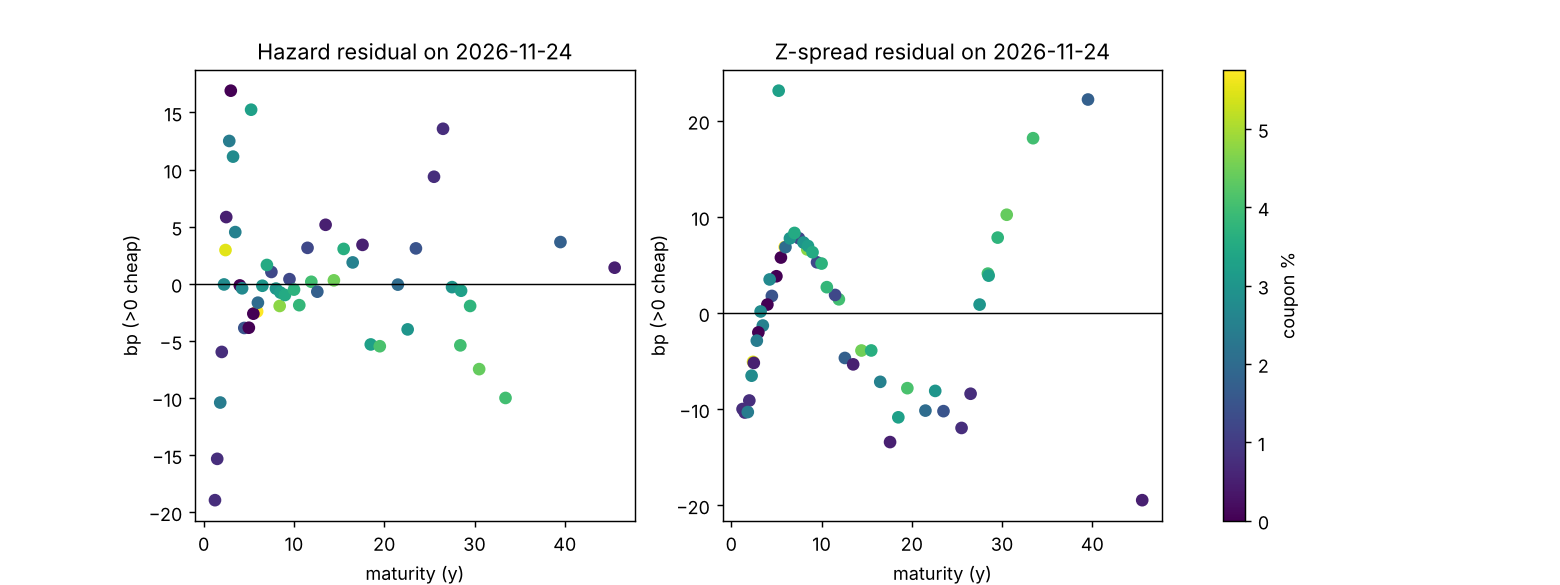
\includegraphics[width=0.95\linewidth]{fig_snapshot.png}\caption{Residuals on the last date, coloured by coupon.}\end{figure}

\section*{Caveats}
\begin{itemize}\itemsep0pt
\item Recovery is assumed; $\lambda$ and $R$ trade off. Re-run with \texttt{--recovery 0.25}.
\item Non-credit effects (liquidity, repo specialness, free float, CTD status) load onto $\lambda$ or the residuals.
\item Coupon dates are maturity anniversaries; irregular first coupons, holidays and business-day rolls ignored.
\item CDS is USD, bonds EUR: the basis includes redenomination/quanto effects.
\end{itemize}
\end{document}
